\documentclass[a4paper]{report}

% Just because I'm too lazy to update the author and title name two places :)
\newcommand{\thisAuthor}{Jan Magne Tjensvold}
\newcommand{\thisTitle}{Generic Distributed Exact Cover Solver}


% Import packages
\usepackage{amsmath, amsfonts, amsthm}  % AMS math libraries
\usepackage{amssymb}       % Large extended set of symbols: http://home.online.no/~pjacklam/latex/textcomp.pdf
\usepackage{multirow}      % Row spanning in tables.
\usepackage{graphicx}      % Extended graphics library
%\usepackage{textcomp}      % Extended set of symbols: http://home.online.no/~pjacklam/latex/textcomp.pdf
%\usepackage{varioref}      % Use \vref instead of \ref
%\usepackage{wrapfig}
%\usepackage{subfigure}
%\usepackage{url}
\usepackage{float}         % Nust be included manually before hyperref so that the algorithm packages work properly.
\usepackage[pdftex,
	pdfauthor={\thisAuthor},
	pdftitle={\thisTitle},
	pdfkeywords={Distributed; Computing; Distributed computing; Exact Cover; Dancing Links; DLX},
	pdfsubject={Distributed computing},
	pdflang={en},
	bookmarks,
	bookmarksnumbered,
]{hyperref}  % Sets pdfTeX to include bookmarks in the output file (Should always be the last package included)
\usepackage[all]{hypcap}   % Links to figures now point at the top of the figure instead of the caption.
\usepackage{algorithm}     % Pseudocode float environment
\usepackage{algorithmic}   % Pseudocode
\usepackage[noend, nobraces]{javadistalgo}  % Java style pseudocode


\graphicspath{{./}{images/}}



% Limit the depth of the table of contents
%\setcounter{tocdepth}{1}

% Custom commands

\renewcommand{\bmod}{\mbox{ mod }}

%\makeatletter
%\def\imod#1{\allowbreak\mkern10mu({\operator@font mod}\,\,#1)}
%\makeatother

%\DeclareMathOperator{\lcm}{lcm}

% Degree symbol for LaTeX and math mode
%\newcommand{\degree}{\ensuremath{^\circ}}

% Some useful environments.
\newenvironment{definition}[1][Definition]{\begin{trivlist}
\item[\hskip \labelsep {\bfseries #1}]}{\end{trivlist}}
\newenvironment{example}[1][Example]{\begin{trivlist}
\item[\hskip \labelsep {\bfseries #1}]}{\end{trivlist}}
\newenvironment{remark}[1][Remark]{\begin{trivlist}
\item[\hskip \labelsep {\bfseries #1}]}{\end{trivlist}}


% Document title page information
\title{\thisTitle}
\author{\thisAuthor}
\date{\today}

% Here the actual document begins.
\begin{document}


\pagenumbering{roman}
\maketitle  % Document title page

\setcounter{page}{2}

\chapter*{Abstract}
\addcontentsline{toc}{chapter}{Abstract}


  % Abstract

% Table of contents, tables and figures
\tableofcontents
%\listoftables
\listoffigures

\cleardoublepage
\pagenumbering{arabic} \setcounter{page}{1}

% Include external files

\chapter{Introduction}


\section{Related work}


\section{Paper organization}

This paper is organized into several chapters. Chapter \ref{dancing_links} describes the Dancing Links algorithm. Chapter \ref{distributed_computing} explains the concept of Grid computing. Chapter \ref{implementation} discusses different aspects of the implementation. Chapter \ref{testing} describes the test results with the system and Chapter \ref{conclusion} concludes this paper.


\section{Architecture}


\begin{figure}[htb]
	\centering 
	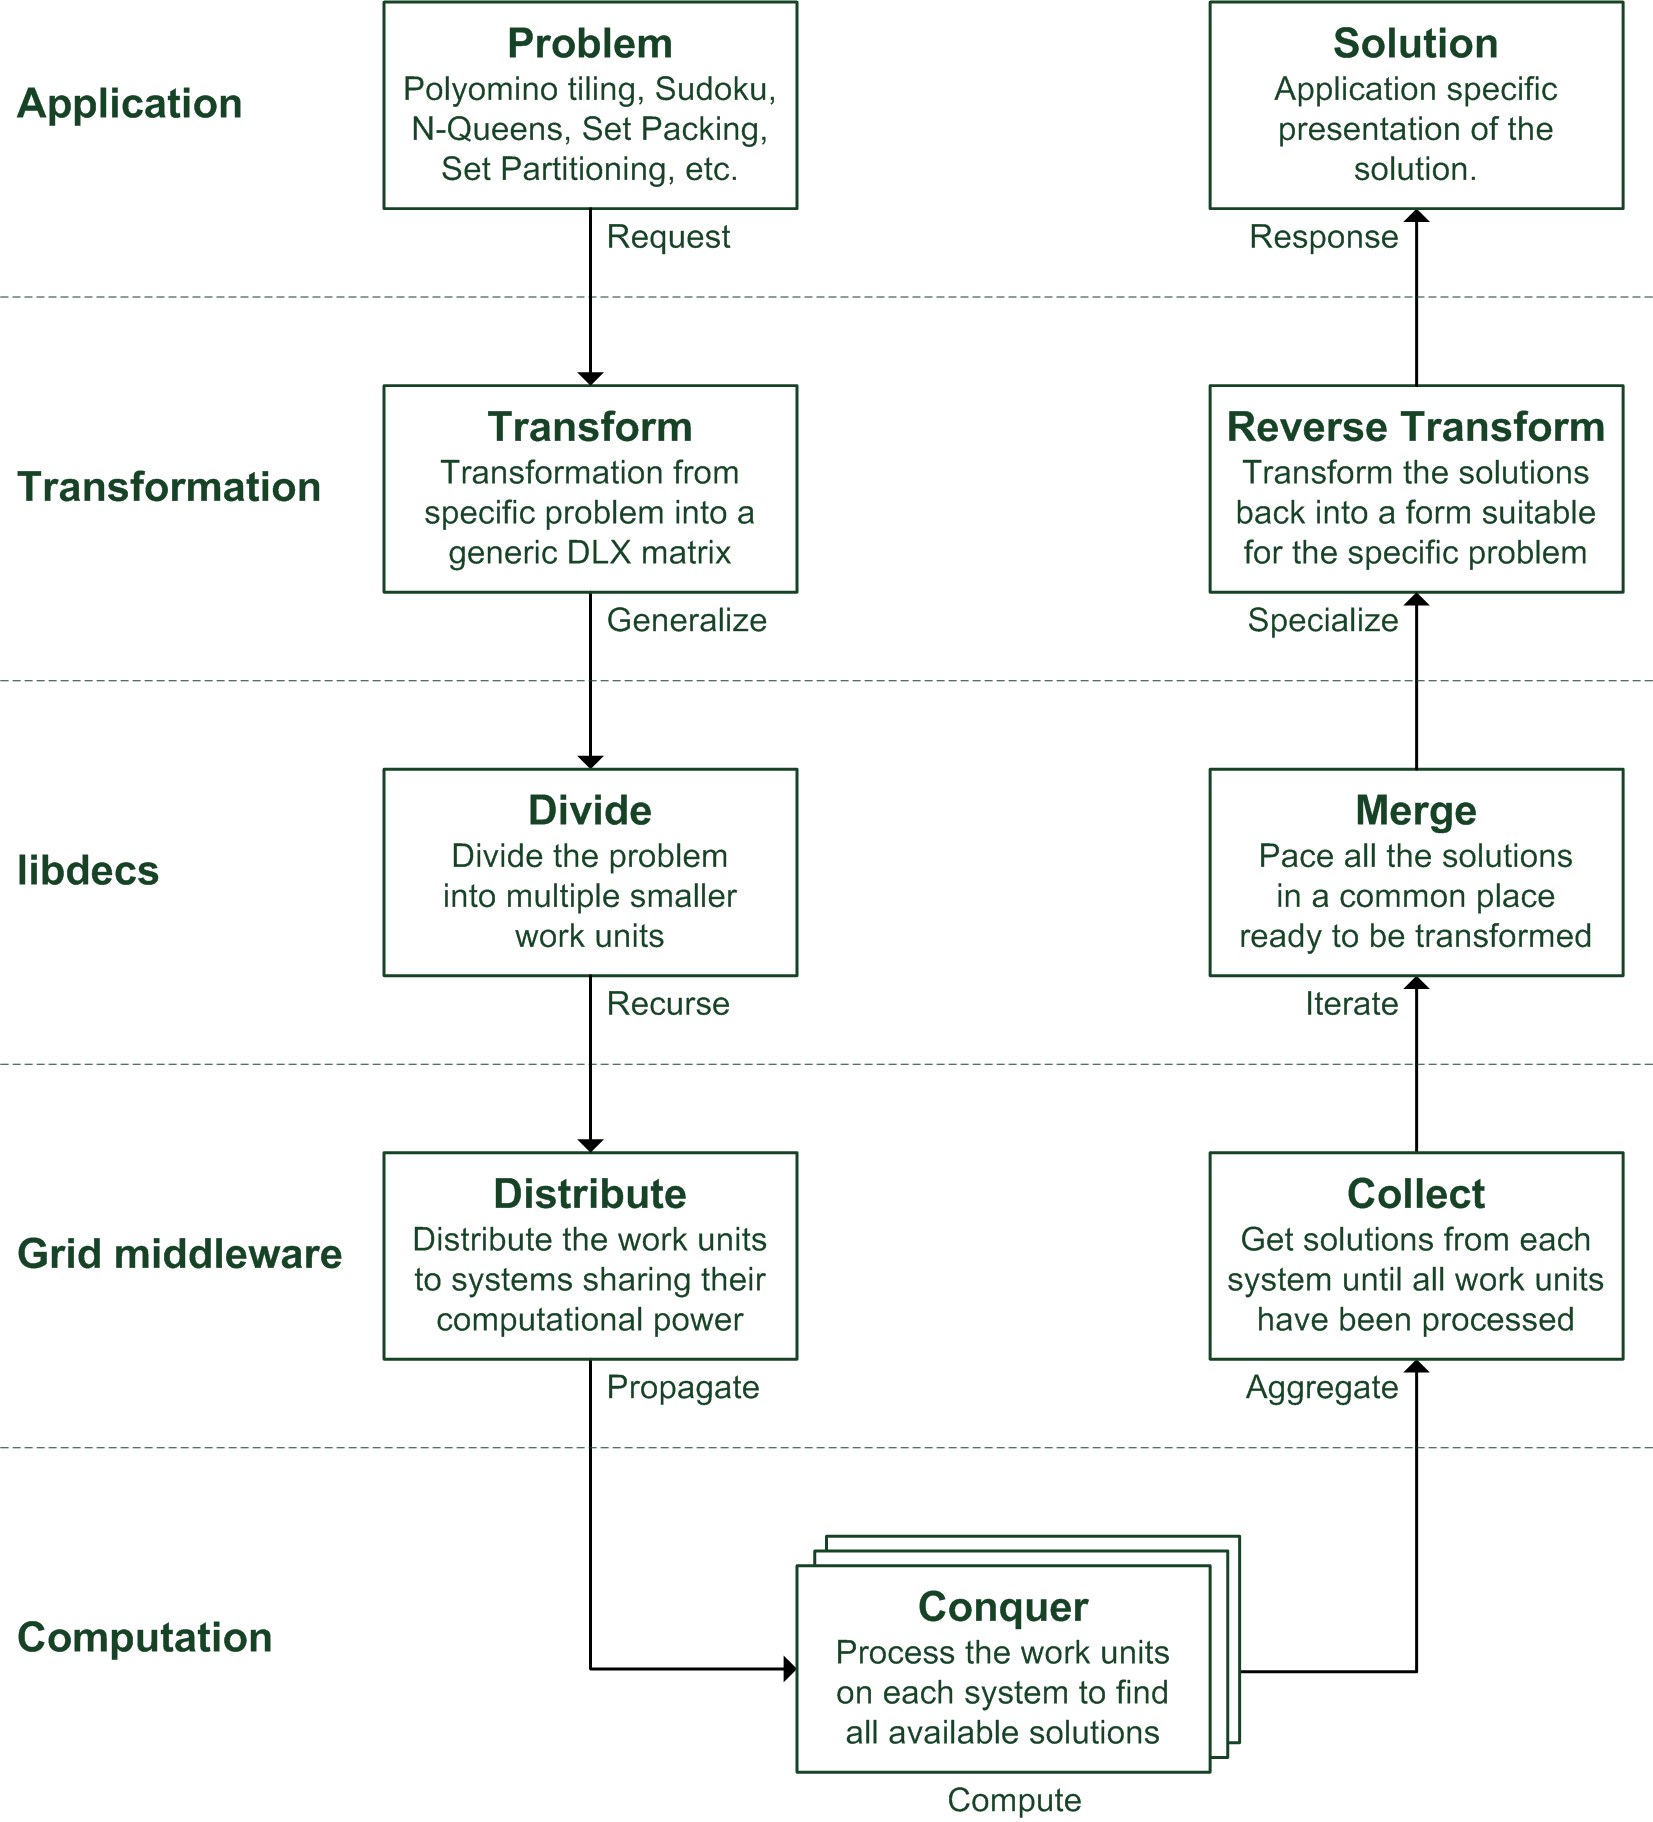
\includegraphics[width=1.0\textwidth]{Architecture.png}
	\caption{Architecture of the Distributed Exact Cover Solver system}
	\label{fig:architecture}
\end{figure}



\chapter{Dancing Links}
\label{dancing_links}

Dancing Links (DLX) is an algorithm invented by Donald Knuth to solve any exact cover problem.
It was first described in \cite{knuth00dancing} where he looks at the details of the algorithm and uses it to solve some practical problems.
Before we look at the DLX algorithm in more detail we need to explain what an exact cover problem is.



\section{Exact cover}
\label{exact_cover}

To represent an exact cover problem we use a matrix in which each element is either zero or one (non-zero).
This type of matrix is called a boolean, binary, logical or \{0,1\}-matrix.
We use ``matrix'' in the rest of this report to mean a boolean matrix and to prevent ambiguity ``non-zero'' is used instead of ``one'' to identify the value of a matrix element\footnote{A non-zero value is effectively the same as one because a boolean matrix can only have elements zero and one.}.

\begin{definition}
Given a collection of subsets $E$ of a set $U$, an exact cover is a subset $S$ of $E$ such that each element of $U$ appears once in $S$.
\end{definition}

The set $U$ is the set of columns $U = \{ 1, 2, \ldots, n \}$.
$E$ is the collection of rows where each set contains the number of the columns which has non-zero values.
The idea is that each column in the matrix represents a specific constraint and each row is a way to satisfy some of the constraints.

For the general $m \times n$ matrix
\[
A =
\left[
\begin{array}{ccccc}
	a_{1,1} & a_{1,2} & a_{1,3} & \cdots & a_{1,n} \\
	a_{2,1} & a_{2,2} & a_{2,3} & \cdots & a_{2,n} \\
	a_{3,1} & a_{3,2} & a_{3,3} & \cdots & a_{3,n} \\
	\vdots  & \vdots  & \vdots  & \ddots & \vdots  \\
	a_{m,1} & a_{m,2} & a_{m,3} & \cdots & a_{m,n} \\
\end{array}
\right]
\]
$a_{i,j}$ is an element in the matrix at row $i$, column $j$ where $a_{i,j} \in \{0,1\}$.
The number of rows is $m$ and the number of columns is $n$.
A subset of rows from a matrix is an exact cover iff (if and only if) each column has exactly one non-zero (one) element.
Let $R_A$ and $R_B$ be the set of rows in matrix $A$ and $B$ respectively.
If $R_B \subseteq R_A$ then $B$ forms the following $k \times n$ matrix
\[
	B =
	\left[
	\begin{array}{ccccc}
		b_{1,1} & b_{1,2} & b_{1,3} & \cdots & b_{1,n} \\
		b_{2,1} & b_{2,2} & b_{2,3} & \cdots & b_{2,n} \\
		b_{3,1} & b_{3,2} & b_{3,3} & \cdots & b_{3,n} \\
		\vdots  & \vdots  & \vdots  & \ddots & \vdots  \\
		b_{k,1} & b_{k,2} & b_{k,3} & \cdots & b_{k,n} \\
	\end{array}
	\right]
\]
$k \leq m$ so that $B$ is a reduced matrix of $A$ or, in the case where $k = m$, the two matrices are identical.
The number of columns in $A$ and $B$ is always the same.
The subset $R_B$ is an exact cover iff the following equation is satisfied
\[
	\sum_{i = 1}^{k} b_{i,j} = 1 \;\;\; \text{for all } j \in \{ 1, 2, \ldots, n \}
\]

\begin{example}
In practical applications we are usually given an initial matrix $A$ and tasked with finding all the subsets of rows which are exact covers.
For example the following matrix
\begin{equation}
	\left[
	\begin{array}{cccc}
		1 & 0 & 0 & 0 \\
		0 & 1 & 1 & 0 \\
		1 & 0 & 0 & 1 \\
		0 & 0 & 1 & 1 \\
		0 & 1 & 0 & 0 \\
		0 & 0 & 1 & 0 \\
	\end{array}
	\right]
	\label{eq:cover_example}
\end{equation}
represents a specific exact cover problem.
In this matrix row 2 and 3 form a valid solution (exact cover) because the subset of rows $\{ 2, 3 \}$, and thus the reduced matrix
\[
\left[
\begin{array}{cccc}
	0 & 1 & 1 & 0 \\
	1 & 0 & 0 & 1 \\
\end{array}
\right]
\]
has exactly one non-zero element in each column.
By adopting a trial and error approach one can find that the full set of solutions for the matrix in (\ref{eq:cover_example}) is $\{ \{1, 4, 5 \}, \{ 2, 3\}, \{ 3, 5, 6\} \}$.
\end{example}


\subsection{Generalized exact cover}

A generalized form of the exact cover problem is sometimes better suited to solve certain types of problems.
The generalized problem can be translated to an exact cover problem by adding additional rows, but translating in the opposite direction is not always possible.
The generalized problem divides the matrix into primary and secondary columns which are subject to two different sets of constraints.
Each primary column in the solution must have exactly one non-zero element, as before.
However, each secondary column in the solution can have either zero or one non-zero element, instead of exactly one.

Let $C_P$ be the set of primary columns and $C_S$ the set of secondary columns in matrix $A$ and $B$.
The subset of rows $R_B$ is an exact cover iff both of the following equations are satisfied
\[
	\sum_{i = 1}^{k} b_{i,j} = 1 \;\;\; \forall j \in C_P  \;\;\;\; \wedge \;\;\;\;  \sum_{i = 1}^{k} b_{i,j} \leq 1 \;\;\; \forall j \in C_S
\]


$n$-queens (see Section \ref{queens_trans}) is one type of problem the generalized cover problem can be applied to.
Creating a secondary column for each diagonal on the chess board will reduce the number of rows in the final matrix.
Given a smaller matrix the DLX algorithm will have to do less processing to find the solutions which results in better performance.
The DLX algorithm itself does not require any modifications to solve generalized cover problems, but the matrix construction procedure requires some minor adjustments (see Section \ref{matrix_construction}).

\begin{example}
In the 4-queens problem each of the four ranks (rows) and four files (columns) on the board corresponds to a primary column in the exact cover matrix.
Each rank and file can only contain one queen, otherwise the queens would attack each other either horizontally or vertically in that rank or file.
Placing 4 queens on a $4 \times 4$ board means that each rank and file must contain exactly one queen.
However, queens can also attack diagonally, but the number of diagonals is larger than the number of queens.
The solution to the 8-queens problem in Figure \ref{fig:8queens} clearly shows that several of the diagonals have no queens.
To model this part of the problem we can use the generalized form of the exact cover problem and assign each diagonal to a secondary column.

Primary columns 1 to 4 represents the ranks 1 through 4, and primary columns 5 to 8 represents the files A to D.
On a $4 \times 4$ board there are ten diagonals if we ignore each of the four corners diagonals, which has only a single square.
The way each diagonal is numbered is unimportant as they are only needed to represent the problem and are not required in order to interpret the final solutions.
We assign each of the ten diagonals to the secondary columns 9 to 18.
Following the exact cover definition the set $U$ is the set of columns $U = \{ 1, 2, \ldots, 18 \}$.
$E$ is the collection of rows where each set contains the column numbers with non-zero elements in that row.
\begin{align*}
C =& \{ \{ 1, 5, 16 \}, \{ 1, 6, 9, 17 \}, \{ 1, 7, 10, 18 \}, \{ 1, 8, 11 \}, \\
&\{ 2, 5, 9, 15 \}, \{ 2, 6, 10, 16 \}, \{ 2, 7, 11, 17 \}, \{ 2, 8, 12, 18 \}, \\
&\{ 3, 5, 10, 14 \}, \{ 3, 6, 11, 15 \}, \{ 3, 7, 12, 16 \}, \{ 3, 8, 13, 17 \}, \\
&\{ 4, 5, 11 \}, \{ 4, 6, 12, 14 \}, \{ 4, 7, 13, 15 \}, \{ 4, 8, 16 \} \}
\end{align*}

Running this though the DLX algorithm provides two solutions $S_1$ and $S_2$.
Notice that in each of the solutions the numbers 1 through 8, which is the primary columns, are present exactly once.
Only eight out of the ten secondary columns are present in the solutions.
Using the first two numbers in each set (the rank and file) we can find out what the solutions look like.
Figure \ref{fig:4queens} shows the board layout of the two solutions.
\begin{align*}
S_1 = \{ \{ 1, 7, 10, 18 \}, \{ 2, 5, 9, 15 \}, \{ 3, 8, 13, 17 \}, \{ 4, 6, 12, 14 \}  \}	\\
S_2 = \{ \{ 1, 6, 9, 17 \}, \{ 2, 8, 12, 18 \}, \{ 3, 5, 10, 14 \}, \{ 4, 7, 13, 15 \}  \}	\\
\end{align*}

\begin{figure}[hptb]
	\centering 
	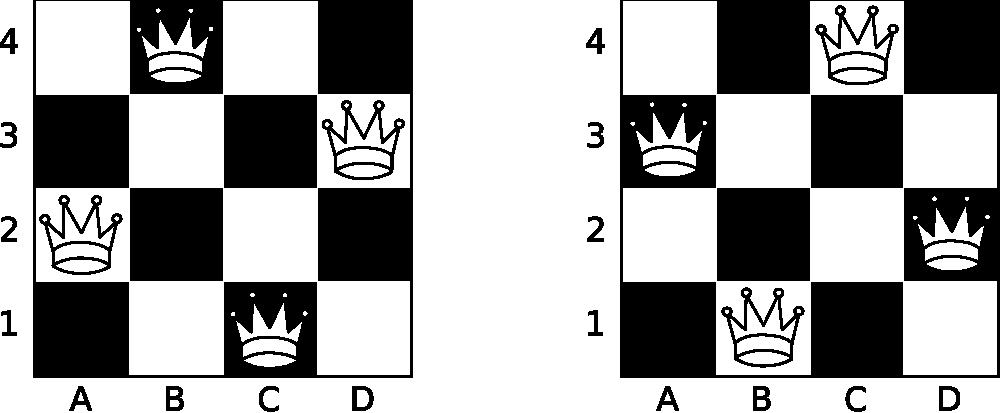
\includegraphics[width=0.79\textwidth]{queens-4x4.pdf}
	\caption{The two solutions $S_1$ (left) and $S_2$ (right) to the 4-queens problem}
	\label{fig:4queens}
\end{figure}

\end{example}


\newpage
\section{Algorithm X}
\label{algox}

Exact cover is a type of problem known to be NP-complete \cite{np-comp-theory}.
Several methods exist which finds all the solutions to an exact cover problem.
optical device
To find all the solutions to an exact cover problem the most straight forward algorithm is to check all possible sets of rows.
Given a set we then check to see if there is exactly one non-zero element in each column.
However, as the size of the matrix increases we will experience a combinatorial explosion on the number of possible sets to test.
The exact number of sets is $2^{m}-1$ given a matrix with $m$ rows.
The 8-queens problem (see Section \ref{queens_trans}) which has a matrix consisting of 63 rows, gives an immense 9~223~372~036~854~775~808 sets.
Given that only 92 of these are valid solutions this simple algorithm can hardly be recommended.

Another approach, which is presented in \cite{knuth00dancing}, is Algorithm X (for the lack of a better name).
This backtrack algorithm uses a more intelligent elimination method to ``wriggle'' its way through the matrix and find all the solutions.
Looking at matrix (\ref{eq:cover_example}) we can easily determine that row 1 and 3 can never be in the same set.
They are in conflict with each other because both of them have a non-zero element in the first column.
Since there must be exactly one non-zero element in each column we can rule out any set containing both row 1 and 3.

Algorithm X uses similar logic to recursively traverse the search tree by backtracking.
Backtracking is the process of exploring all possible paths in a search tree to locate solutions.
When a path in the search does not yield any solutions the algorithm backtracks and starts searching the next available path in the tree.
A modified version of Algorithm X is presented in Algorithm \ref{alg:algox}.
Changes are made to improve the readability, logical consistency and to make it easier to compare with the Dancing Links algorithm.
Algorithm X is initially called with the matrix $A$ and the column header list $H$.
$H$ is initialized with the numbers $1, 2, \ldots, n$, where $n$ is the number of columns in $A$.

\begin{algorithm}[htbp]
	\caption{Algorithm X recursive search procedure.}
	\label{alg:algox}
	\begin{distribalgo}[1]
		\PROCEDURE{search($A, H$)}
			\IF{$H$ is empty}
				\STATE Print solution and return.  \COMMENT{Base case for the recursion}
			\ENDIF
			\STATE Choose a column $c$.
			\FOREACH{row $r$ such that $a_{r,c} = 1$}
				\STATE Add $r$ to partial solution.
				\STATE Save state of matrix $A$ and list $H$.
				\FOREACH{column $j$ such that $a_{r,j} = 1$}
					\FOREACH{row $i$ such that $a_{i,j} = 1$, \textbf{except} $i = r$}
						\STATE Delete row $i$ from matrix $A$.
					\ENDFOR
					\STATE Delete column $j$ from matrix $A$ and list $H$.
				\ENDFOR
				\STATE Delete row $r$ from matrix $A$.
				\STATE search($A,H$)
				\STATE Restore state of matrix $A$ and list $H$.
				\STATE Remove $r$ from the partial solution.
			\ENDFOR
		\ENDPROC
	\end{distribalgo}
\end{algorithm}

If $H$ is empty the partial solution is an exact cover and the algorithm returns.
Otherwise, the algorithm chooses a column $c$ and loops through each row $r$ which has a non-zero element in column $c$.
Any conflict between row $r$ and the remaining rows are resolved at line 8 to 12.
The algorithm then calls itself recursively with the reduced matrix and column list.
This continues until all the rows with non-zero elements in column $c$ have been tested, in which case all the branches in the search tree have been traversed.

Any rule for choosing column $c$ will produce all the solutions, but there are some rules that work better than others.
In \cite{knuth00dancing} Knuth uses what he refers to as the $S$ heuristic, which is to always choose the column with the least amount of non-zero elements.
This approach has proved to work well in a large number of cases so it is a reasonable rule to make use of in practice.

\begin{example}
Using matrix (\ref{eq:cover_example}) we wish to demonstrate how Algorithm X works.
The columns and rows have been numbered to make it easier to keep track of them when the matrix is modified.
\begin{equation*}
	\label{eq:ces1}
	\begin{array}{r} 1\\ 2\\ 3\\ 4\\ 5\\ 6 \end{array}
	\stackrel{
		\begin{array}{cccc} 1 & 2 & 3 & 4 \end{array}
	}{
		\begin{bmatrix}
			1 & 0 & 0 & 0 \\
			0 & 1 & 1 & 0 \\
			1 & 0 & 0 & 1 \\
			0 & 0 & 1 & 1 \\
			0 & 1 & 0 & 0 \\
			0 & 0 & 1 & 0 \\
		\end{bmatrix}
	}
\end{equation*}
We begin by choosing column 1.
Looking at this column we choose row 1 where there is a non-zero element.
Our partial solution is now $\{ 1 \}$.
Row 1 only has one conflicting row which is row 3, which has a conflict in column 1.
We remove column 1, row 1 and row 3 which results in the following matrix
\begin{equation}
	\label{eq:ces2}
	\begin{array}{r} 2\\ 4\\ 5\\ 6 \end{array}
	\stackrel{
		\begin{array}{ccc} 2 & 3 & 4 \end{array}
	}{
		\begin{bmatrix}
			1 & 1 & 0 \\
			0 & 1 & 1 \\
			1 & 0 & 0 \\
			0 & 1 & 0 \\
		\end{bmatrix}
	}
\end{equation}
This time we choose column 2 and then row 2 so that the partial solution becomes $\{ 1, 2 \}$.
Row 2 conflicts with all the remaining rows (row 5 in column 2 and row 4 and 6 in column 3).
After all the conflicts have been resolved the matrix itself is empty, but the column list $H$ is not.
Because there are no non-zero elements left in the matrix the recursive call will return immediately (the loop condition at line 5 is not satisfied) and matrix (\ref{eq:ces2}) is restored.
This time we choose row 5 which results in the partial solution $\{ 1, 5 \}$.
Row 5 conflicts with row 2 in column 2 and by eliminating the conflicts we get the following matrix
\begin{equation*}
	\label{eq:ces3}
	\begin{array}{r} 4\\ 6 \end{array}
	\stackrel{
		\begin{array}{ccc} 3 & 4 \end{array}
	}{
		\begin{bmatrix}
			1 & 1 \\
			1 & 0 \\
		\end{bmatrix}
	}
\end{equation*}
We choose column 3 and then row 4 which gives us the partial solution $\{ 1, 5, 4 \}$.
After all the conflicts are resolved the matrix is completely empty along with the column header list.
This tells us that $\{ 1, 5, 4 \}$ is one of the solutions to this problem.

The search tree in Figure \ref{fig:ex_tree} emerges as we continue in the same manner, until all the solutions have been found.
Each node $i,j$, for row $i$ and column $j$, indicates the choices made by the algorithm.
The rectangular nodes is where each of the solutions were found.
The search tree is a binary tree as a result of the small matrix used in this example so this behavior cannot be generalized.
\begin{figure}[htbp]
	\centering 
	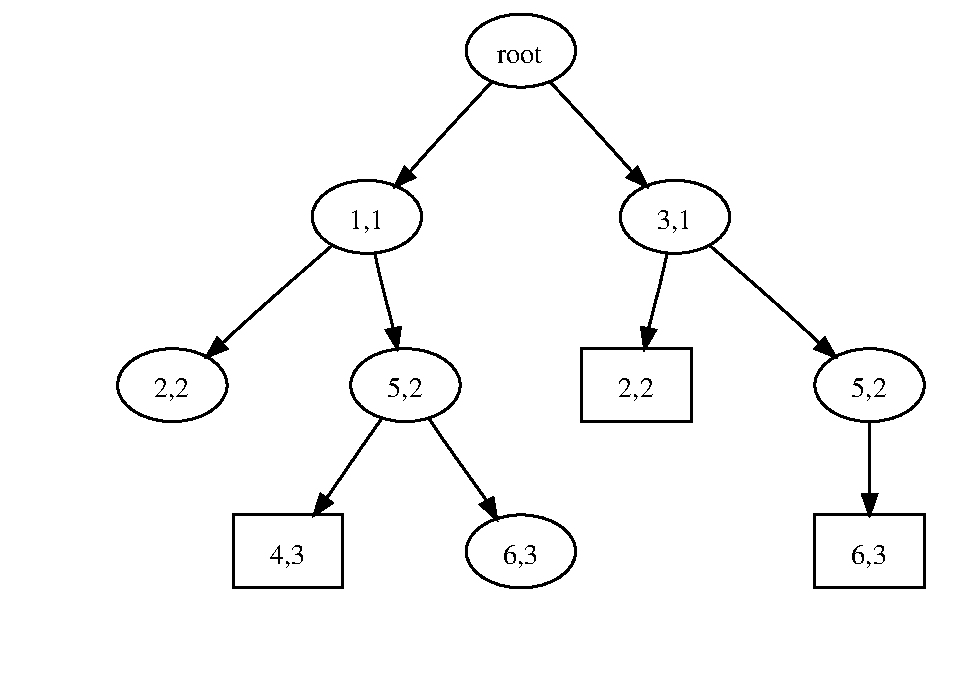
\includegraphics[width=0.85\textwidth]{search-tree-ex.pdf}
	\caption{Algorithm X search tree for the example matrix}
	\label{fig:ex_tree}
\end{figure}

\end{example}

One issue when trying to implement Algorithm X is that the state of the matrix needs to be saved and restored multiple times during the backtrack process.
Each time the algorithm returns the old state must be restored before another path can be explored.
Searching through the matrix to find the non-zero elements is also very time consuming if the matrix is stored as a two dimensional array.
To solve these problems the Dancing Links algorithm was introduced.



\section{Dancing Links}
\label{dlx}

The Dancing Links (DLX) algorithm is based on Algorithm X, but it contains some significant modifications which makes it more suitable for practical applications.
DLX is based on a simple, yet powerful, technique which allows one to reverse any operation made to a doubly-linked list.
If $x$ represents an element in such a list then $x.left$ and $x.right$ points to the previous and next element respectively.
To remove element $x$ from the list the following two operations are applied:
\begin{equation}
	\label{eq:remove}
	\begin{array}{rcl}
		x.right.left &\leftarrow& x.left \\
		x.left.right &\leftarrow& x.right \\
	\end{array}
\end{equation}

Applying these two operations to the linked list in Figure \ref{fig:linked} results in the list in Figure \ref{fig:linked_del}.
These operations modify the links pointing to element $x$ so that an iteration through the list will no longer traverse through this element, but instead skip right past it.
\begin{figure}[htbp]
	\centering 
	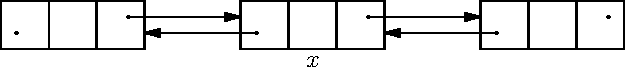
\includegraphics[width=0.8\textwidth]{doubly-linked-list.pdf}
	\caption{Doubly-linked list}
	\label{fig:linked}
\end{figure}
\begin{figure}[htbp]
	\centering 
	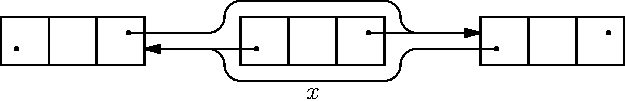
\includegraphics[width=0.8\textwidth]{doubly-linked-list-del.pdf}
	\caption{Doubly-linked list with element $x$ removed}
	\label{fig:linked_del}
\end{figure}

When programming one might be tempted to set $x.left$ and $x.right$ to a null value and delete the $x$ object or let the garbage collector do its thing.
However, smart as that might seem it would prevent one from applying a second set of operations.
In \cite{Hitotumatu79} Hitotumatu and Noshita introduced a pair of operations which allows one to insert an element back into the list in exactly the same place it was removed from.
The following two operations work as the inverse of the operations in (\ref{eq:remove}) by adding $x$ back into the list.
\begin{equation}
	\label{eq:add}
	\begin{array}{rcl}
		x.right.left &\leftarrow& x \\
		x.left.right &\leftarrow& x \\
	\end{array}
\end{equation}

To maintain the state information for the matrix the DLX algorithm uses the operations in (\ref{eq:remove}) and (\ref{eq:add}).
The $x$ element is preserved so that the algorithm can reverse the remove operations, which are used to reduce the matrix.


\subsection{Data structure}
\label{dlx_struct}

DLX stores the matrix as a collection of several circular doubly-linked lists where each non-zero value in the matrix is an element in the lists.
Using this sparse matrix representation saves a lot of memory because the number of zero elements usually outnumber the non-zero elements.
This advantage will normally grow when the size of the matrix increases.
As an example the $n$-queens problem for $n=10$ has 396 non-zero elements, but they only account for 7.33\% of the total number of elements.
% TODO Add density graph/table

Each row and column in the matrix is represented by a separate list.
In addition the set of column headers is also stored in a list.
Each element $x$ in the linked lists have six attributes: $x.left$, $x.right$, $x.up$, $x.down$, $x.column$ and $x.row$.
The $x.row$ attribute is an addition to Knuth's original algorithm to enable detection of the row number.
The first four attributes contains a pointer to an element in the respective list.
$x.left$ and $x.right$ belongs to a row list and $x.up$ and $x.down$ belongs to a column list.
$x.column$ is a pointer to the column header and $x.row$ is a non-negative integer storing the row number of the element.
A column header $c$ has the additional $c.name$ (column name/number) and $c.size$ (number of elements in column) attributes.
Secondary column headers used by the generalized cover problem have their $c.left$ and $c.right$ attributes pointing to $c$ (itself).
The special column header element $h$ acts as a root element for the rest of the data structure.

Figure \ref{fig:matrix_links} shows shows how the matrix in (\ref{eq:cover_example}) can be represented using this data structure.
To avoid clutter the $x.column$ links pointing to the column headers are not displayed in the figure.
\begin{figure}[htbp]
	\centering
	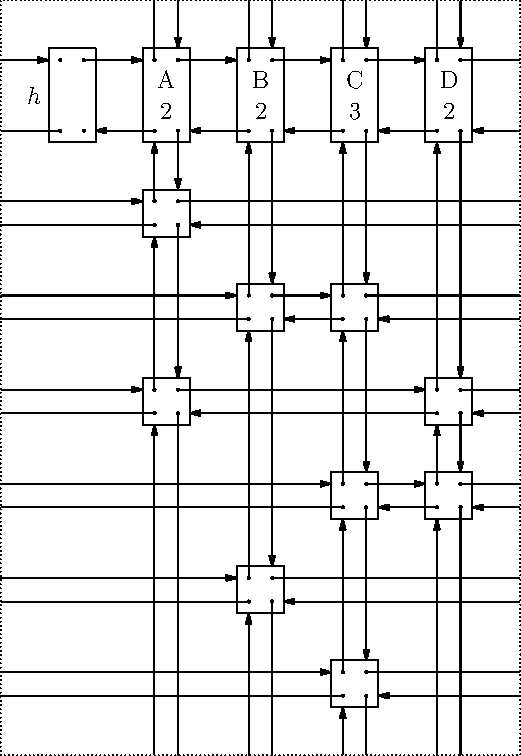
\includegraphics[width=0.52\textwidth]{matrix-links.pdf}
	\caption{Sparse boolean matrix circular quad-linked list representation of the example matrix}
	\label{fig:matrix_links}
\end{figure}


\subsection{Algorithm}

The DLX algorithm is very similar in nature to Algorithm X and in essence the two algorithms work exactly in the same way.
Given the example matrix (\ref{eq:cover_example}) the DLX algorithm will follow the same path as shown in Figure \ref{fig:ex_tree}.
The difference is that DLX uses a specialized data structure together with the linked list remove and add operations to save and restore the state of the matrix.
Comparing Algorithm \ref{alg:algox} and Algorithm \ref{alg:search} reveals that they are very similar in nature.

The DLX algorithm is initially called with $k = 0$ (recursion level 0) and a pointer to the column header $h$ of the matrix.
Printing a solution using the $x.row$ attribute is done by printing $O_{i}.row$ for all $i \in \{1, 2, \ldots, k\}$.
Column selection is done using the $S$ heuristic, which picks the column with the lowest value for $c.size$.
Algorithm \ref{alg:column} simply steps through each column header looking for the lowest size.

\begin{algorithm}[htbp]
	\caption{Dancing Links recursive search.}
	\label{alg:search}
	\begin{distribalgo}[1]
		\PROCEDURE{search($k$)}
			\IF{$h.right = h$}
				\STATE Print solution and return.  \COMMENT{Base case for the recursion}
			\ENDIF
			\STATE $c \leftarrow$ choose\_column()
			\STATE cover($c$)
			\FOREACH{$r \leftarrow c.down, c.down.down, \ldots,$ \textbf{while} $r \neq c$}
				\STATE $O_k \leftarrow r$  \COMMENT{Add $r$ to partial solution}
				\FOREACH{$j \leftarrow r.right, r.right.right, \ldots,$ \textbf{while} $j \neq r$}
					\STATE cover($j.column$)
				\ENDFOR
				\STATE search($k + 1$)
				\FOREACH{$j \leftarrow r.left, r.left.left, \ldots,$ \textbf{while} $j \neq r$}
					\STATE uncover($j.column$)
				\ENDFOR
			\ENDFOR
			\STATE uncover($c$)
		\ENDPROC
	\end{distribalgo}
\end{algorithm}

\begin{algorithm}[htbp]
	\caption{Column selection using the $S$ heuristic.}
	\label{alg:column}
	\begin{distribalgo}[1]
		\FUNCTION{choose\_column()}
			\STATE $s \leftarrow \infty$
			\FOREACH{$j \leftarrow h.right, h.right.right, \ldots,$ \textbf{while} $j \neq h$}
				\IF{$j.size < s$}
					\STATE $c \leftarrow j$
					\STATE $s \leftarrow j.size$
				\ENDIF
			\ENDFOR
			\RETURN{column $c$}
		\ENDFUNC
	\end{distribalgo}
\end{algorithm}

The cover($c$) and uncover($c$) algorithms are the main differences between DLX and Algorithm X.
The purpose of cover($c$) is to remove column $c$ from the column header list and to resolve any conflicts in the column.
It uses the operations in (\ref{eq:remove}) to remove the conflicting elements from the column lists.
The cover($c$) algorithm also increments the value of $updates$ which is used to measure how many operations the search algorithm requires to complete.
One update equals four link modifications or one application of both the linked list remove and add operations.
The $size$ column header attribute is maintained by both the cover($c$) and uncover($c$) algorithms so that the $S$ heuristic works properly.
Algorithm \ref{alg:cover} contains the pseudo code for the cover procedure.
\begin{algorithm}[htbp]
	\caption{Cover column $c$.}
	\label{alg:cover}
	\begin{distribalgo}[1]
		\PROCEDURE{cover($c$)}
			\STATE $c.right.left \leftarrow c.left$  \COMMENT{Remove column $c$}
			\STATE $c.left.right \leftarrow c.right$
			\FOREACH{$i \leftarrow c.down, c.down.down, \ldots,$ \textbf{while} $i \neq c$}
				\FOREACH{$j \leftarrow i.right, i.right.right, \ldots,$ \textbf{while} $j \neq i$}
					\STATE $j.down.up \leftarrow j.up$  \COMMENT{Remove element $j$}
					\STATE $j.up.down \leftarrow j.down$
					\STATE $j.column.size \leftarrow j.column.size - 1$
					\STATE $updates \leftarrow updates + 1$
				\ENDFOR
			\ENDFOR
		\ENDPROC
	\end{distribalgo}
\end{algorithm}

The uncover($c$) algorithm restores the state of the matrix using the operations in (\ref{eq:add}).
Notice that Algorithm \ref{alg:uncover} walks up and left in the lists while Algorithm \ref{alg:cover} walks down and right.
This ensures that the elements are put back in the reverse order in which they were removed.
This is the only way to make sure that all the links are restored to their original state.
\begin{algorithm}[htbp]
	\caption{Uncover column $c$.}
	\label{alg:uncover}
	\begin{distribalgo}[1]
		\PROCEDURE{uncover($c$)}
			\FOREACH{$i \leftarrow c.up, c.up.up \ldots,$ \textbf{while} $i \neq c$}
				\FOREACH{$j \leftarrow i.left, i.left.lseft, \ldots,$ \textbf{while} $j \neq i$}
					\STATE $j.column.size \leftarrow j.column.size + 1$
					\STATE $j.down.up \leftarrow j$  \COMMENT{Add element $j$}
					\STATE $j.up.down \leftarrow j$
				\ENDFOR
			\ENDFOR
			\STATE $c.right.left \leftarrow c$  \COMMENT{Add column $c$}
			\STATE $c.left.right \leftarrow c$
		\ENDPROC
	\end{distribalgo}
\end{algorithm}



\section{Parallel Dancing Links}

To be able to solve more complex exact cover problems the solution process must be distributed to a larger number of computers.
To accomplish this we must first break the problem into smaller pieces.
In \cite{maus-prp} Maus and Aas investigates recursive procedures as the unit for parallelizing.
They introduce some techniques on how to split the recursion tree which can be directly applied to the search tree in DLX.
The main idea is that the algorithm is first run in a breath-first mode so that the search tree is explored one level at a time.
When a certain number of nodes in the tree has been discovered the search stops and the nodes are distributed to a set of computers and solved in parallel.

The search procedure of DLX is a backtrack algorithm which explores the search tree depth-first.
Making this a breath-first algorithm can be achieved by not allowing it to proceed deeper than a certain level in the search tree.
When the given level is reached the partial solution $O$ is saved.
$O$ can then be used to initialize a separate process by running DLX on a different computer (or another processor on the same computer).
As long as the predefined depth $d$ is not too deep or shallow the partial solutions can be used to efficiently solve the exact cover problem in a distributed manner.
If $d$ is too deep (high) the algorithm will find all solutions before the splitting happens, and if it is too shallow (low) the number of partial solutions might be too low to be of any use.
Adding line 10 to 12 in Algorithm \ref{alg:psearch} is the only changes required to make the original Algorithm \ref{alg:search} support this scheme.
\begin{algorithm}[htbp]
	\caption{Dancing Links parallel recursive splitter.}
	\label{alg:psearch}
	\begin{distribalgo}[1]
		\PROCEDURE{psearch($k, d$)}
			\IF{$h.right = h$}
				\STATE Print solution and return.  \COMMENT{Base case for the recursion}
			\ENDIF
			\STATE $c \leftarrow$ choose\_column()
			\STATE cover($c$)
			\FOREACH{$r \leftarrow c.down, c.down.down, \ldots,$ \textbf{while} $r \neq c$}
				\STATE $O_k \leftarrow r$  \COMMENT{Add $r$ to partial solution}
				\FOREACH{$j \leftarrow r.right, r.right.right, \ldots,$ \textbf{while} $j \neq r$}
					\STATE cover($j.column$)
				\ENDFOR
				\IF{$k \geq d$ and $h.right \neq h$}
					\STATE Print partial solution.  \COMMENT{Prevent further recursion}
				\ELSE
					\STATE psearch($k + 1$)
				\ENDIF
				\FOREACH{$j \leftarrow r.left, r.left.left, \ldots,$ \textbf{while} $j \neq r$}
					\STATE uncover($j.column$)
				\ENDFOR
			\ENDFOR
			\STATE uncover($c$)
		\ENDPROC
	\end{distribalgo}
\end{algorithm}

Each partial solution produced by psearch($k, d$) can be used as an initialization vector for the modified search procedure search\_init($O$) in Algorithm \ref{algo:isearch}.
$O$ is the initialization vector and $O.size$ is the length of the vector (number of rows in the partial solution).
The initialization vectors and the matrix can be distributed and the modified search procedure can be run in parallel on each computer.
If required each computer can do further splitting locally to take advantage of multiple processors.
\begin{algorithm}[htbp]
	\caption{Dancing Links search initialization.}
	\label{algo:isearch}
	\begin{distribalgo}[1]
		\PROCEDURE{search\_init($O$)}
			\FOR{$k \leftarrow 0$ \textbf{to} $O.size - 1$}
				\STATE $c \leftarrow$ choose\_column()
				\STATE cover($c$)
				\STATE $r \leftarrow O_k$
				\FOREACH{$j \leftarrow r.right, r.right.right, \ldots,$ \textbf{while} $j \neq r$}
					\STATE cover($j.column$)
				\ENDFOR
			\ENDFOR
			\STATE search($O.size$)  \COMMENT{Do actual search}
		\ENDPROC
	\end{distribalgo}
\end{algorithm}

This approach does not guarantee that each initialization vector provides the same amount of work.
Unfortunately there is no straight forward method to estimate the complexity of the subtree given by a specific initialization vector.
In \cite{knuth75backtracking} Knuth uses a Monte Carlo approach to estimate the running time of a backtrack algorithm.
By doing random walks in the subtree he is able to estimate the cost of backtracking.
This approach would be worth investigating for a future version of DECS.

\chapter{Implementation details}
\label{implementation}
% Here we describe some of the important implementation details.

DECS has been implemented in the C++ programming language and the source code is available at \url{http://decs.googlecode.com/} licensed under the GNU General Public License version 2.
The DECS software suite consists of several parts:
\begin{description}
	\item[libdecs]
		This static library contains all the essential parts of DECS like the DLX algorithm, the sparse boolean matrix representation code and the file input/output functionality.
	\item[dance]
		The dance command line program can solve exact covers stored in the DECS file format.
		It can also display various information about the content of a DECS file.
	\item[bdance]
		The bdance program is integrated with the BOINC framework.
		This is the program that any BOINC client connected to the DECS project will download and use.
		It simply reads from the file in.decs, solves the exact cover and writes the solutions to the out.decs file.
	\item[degen]
		The DECS matrix generator is a command line program which can build exact cover matrices and save them in the DECS file format.
		It can also do reverse transforms and analyze DECS result files from previous computations.
		It relies on a set of libraries to do forward and reverse transforms on the specific type of problem.
		Currently the only library available is for the $n$-queens problem.
\end{description}



\section{Architecture}

\begin{figure}[htbp]
	\centering 
	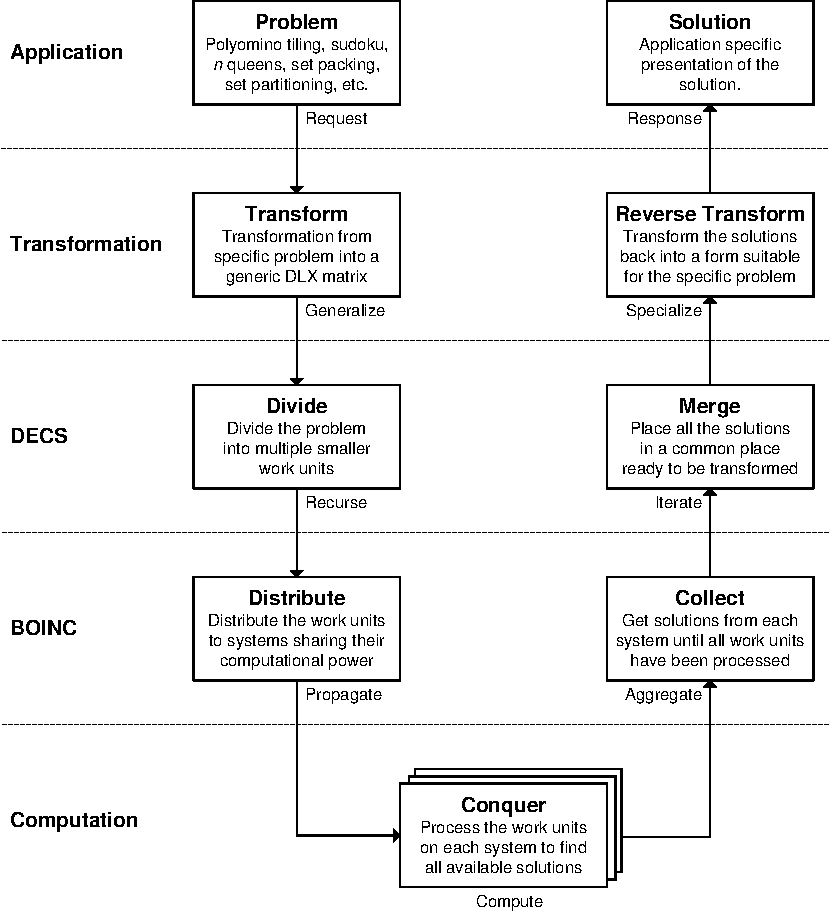
\includegraphics[width=1.0\textwidth]{architecture.pdf}
	\caption{Generic Distributed Exact Cover Solver system architecture}
	\label{fig:architecture}
\end{figure}

The DECS system architecture is layer based as shown in Figure \ref{fig:architecture}.
The application layer is where external applications produce exact cover problems and where the final solutions end up.
The transformation layer is where the degen program and its libraries operate.
The generalization step is when degen receives a problem, turns it into an exact cover problem and outputs the matrix in the DECS file format.
This file is then handed to libdecs where the DLX parallel recursive splitter (Algorithm \ref{alg:psearch}) produces a number of work units.
Each of the work units are handed to the BOINC system, which makes sure that they are available for clients connected to the BOINC server provided by DECS.
When a client receives a work unit it runs the DLX algorithm (Algorithm \ref{alg:isearch}) to find all the solutions.
The client then sends the solutions back the the BOINC server where they are verified for correctness and stored until the solutions to all the related work units has been received.
BOINC then hands the solutions back to libdecs which reads and analyzes the solution files and merges them into a single file.
Finally it passes the resulting file to the degen program which runs a reverse transform on the solutions.
It then writes the final results in whatever format the application needs.



%\section{BOINC}

% TODO: Important - Write more about BOINC.
%\subsection{Architecture}

%Components of a BOINC server
%\begin{itemize}
%	\item Feeder
%	\item Transitioner
%	\item File deleter
%	\item Application
%	\item Work generator
%	\item Validator
%	\item Assimilator
%\end{itemize}

% To keep track of the different files and work units BOINC renames them and keeps track of them by storing their names in a database.



\section{Transforms}
\label{transforms}

To turn a specific problem into an exact cover problem an algorithm is needed that understands that specific problem.
This algorithm then turns the problem into an exact cover matrix which can be solved by the DLX algorithm.
When the solutions to the matrix has been found they need to be translated back (reverse transform) into the domain of the original problem so that it is possible to understand the end result.
The degen program makes use of a set of libraries to accomplish these two task.


\subsection{\texorpdfstring{$n$}{n}-queens}
\label{queens_trans}

The $n$-queens problem has been described in detail in Section \ref{intro_queens} along with an example in Section \ref{general_exact_cover}.
It was originally proposed by the chess player Max Bezzel in 1848.
Since that time many people has made an effort to find the number of solutions for steadily increasing values of $n$.
The next unsolved puzzle is for $n = 26$ which is expected to have somewhere around $2 \times 10^{16}$ solutions.
Trying to parallelize the $n$-queens problem is nothing new.
As early as 1989 Bruce Abramson and Moti Yung presented a divide and conquer algorithm in \cite{Abramson89} which in principle could be used to do parallel processing.
A Danish bachelor project from the spring of 2007 \cite{queens-mig} tried to solve the problem for $n=26$ on the MiG \cite{mig} Grid computing platform.
One of the most promising projects lately is the BOINC based NQueens@Home \cite{nqueensathome} project.
About 13 years of CPU time has been registered by the project after running for only 3 months.

Algorithm \ref{alg:nqeens-cover} shows how the $n$-queens transform takes place.
The parameter $A$ is a matrix (or two dimmensional array) with all elements set to zero, $i \times j$ rows, $2n$ primary columns and $4n - 6$ secondary columns (for the two diagonals).
The elements in $A$ are accessed by $A[i,j]$ where $i$ is the row, $j$ is the column and both values start at zero.
Each iteration through the inner loop generates one row in the matrix for each file on the chessboard.
The outer loop steps through all the ranks on the board and by multiplying the number of ranks and files we get $n^2$ rows in the final matrix.
Each of these rows represents a unique placement of a queen on the chessboard.
The algorithm is made a bit complex by the calculation of each of the two diagonals.
At the end of the algorithm the matrix $A$ can be saved to file and made ready for further processing.
\begin{algorithm}[H]
	\caption{Transforming $n$-queens into the exact cover matrix $A$.}
	\label{alg:nqeens-cover}
	\algsetup{indent=6mm}
	\begin{distribalgo}[1]
		\PROCEDURE{queens-tf($n$, $A$)}
			\FOR{$i \leftarrow 0$ \textbf{to} $n - 1$}
				\FOR{$j \leftarrow 0$ \textbf{to} $n - 1$}
					\STATE $row \leftarrow i \times j$
					\STATE $A[row,i] \leftarrow 1$  \COMMENT{The rank}
					\STATE $A[row,j+n] \leftarrow 1$  \COMMENT{The file}
					\STATE $d_1 \leftarrow i + j$  \COMMENT{The first diagonal}
					\IF{$d_1 \neq 0$ and $d_1 \neq 2n - 2$}
						\IF{$d_1 < 2n - 2$}
							\STATE $A[row,d_1 + 2n - 1] \leftarrow 1$
						\ELSE
							\STATE $A[row,d_1 + 2n - 2] \leftarrow 1$
						\ENDIF
					\ENDIF
					\STATE $d_2 \leftarrow n - i + j - 1$  \COMMENT{The second diagonal}
					\IF{$d_2 \neq 0$ and $d_2 \neq 2n - 2$}
						\IF{$d_2 < 2n - 2$}
							\STATE $A[row,d_2 + 4n - 4] \leftarrow 1$
						\ELSE
							\STATE $A[row,d_2 + 4n - 5] \leftarrow 1$
						\ENDIF
					\ENDIF
				\ENDFOR
			\ENDFOR
		\ENDPROC
	\end{distribalgo}
\end{algorithm}
\noindent Algorithm \ref{alg:nqeens-reverse} shows how to place the queens on the $8 \times 8$ chessboard when a solution has been found.
The input parameters to the algorithms is the solution $S$, which is a set of row numbers, and the number of queens $n$.
It uses zero based row numbers and provides zero based rank and file values as a result.
\begin{algorithm}[H]
	\caption{Reverse transforming $n$-queens to chessboard placements.}
	\label{alg:nqeens-reverse}
	\algsetup{indent=6mm}
	\begin{distribalgo}[1]
		\PROCEDURE{queens-rtf($S, n$)}
			\FOREACH{row $i$ in $S$}
				\STATE $f \leftarrow i \bmod n$
				\STATE $r \leftarrow (i - f) / n$
				\STATE Place a queen at file $f$ and rank $r$.
			\ENDFOR
			\STATE Show chessboard.
		\ENDPROC
	\end{distribalgo}
\end{algorithm}

\begin{example}
Using the dance program to solve the 8-queens problem gives us a list of 92 solutions like this
\begin{verbatim}
$ dance --verbose examples/queens8.decs
[...]
Solution: 3 15 20 26 49 61 32 46
[...]
Search complete

Number of solutions: 92
\end{verbatim}
The solutions contains the row numbers from the matrix and not the entire content of the rows.
The row numbers given in the output are zero based.
Using the reverse transform algorithm above with $S = \{3, 15, 20, 26, 49, 61, 32, 46\}$ and $n = 8$ the queens are placed on the chessboard where they belong.
Working though the list of rows reveals the same chessboard as shown in Figure \ref{fig:8queens}.
\end{example}




%\subsection{Polyominoes}
%\label{poly_trans}

%Solomon W. Golomb practically invented the concept of polyominoes and made it widely available in his book \cite{Polyominoes}.


%\subsection{Latin square}
%\label{latin_trans}

%\cite{Colbourn04}
% Application of Exact Cover to Solving the Latin Square Puzzle
% -- http://www.imtek.de/simulation//mathematica/IMSweb/imsTOC/Game%20Theory/ExactCoverDocu.html

%Latin square puzzles - Special types of Latin squares can be used as error correcting codes for power line communication (sending radio signals over electric power lines) \cite{Colbourn04}


%\subsection{Sudoku}
%\label{sudoku_trans}

% Sudoku (special case of Latin squares)
%Granted Sudoku 



\section{File format}

In order to store and transfer a DLX problem matrix efficiently a file format had to be defined for this specific purpose.


\subsection{Byte ordering}

Several challenges arise when defining a file format, but one of the most common is that of byte ordering.
Different platforms use different byte ordering, meaning that the order of the bytes in variables bigger than 1 byte may differ from one system to another.

Byte ordering deals with how the bytes for individual variables are ordered in memory.
For a 1 byte large variable the byte ordering is irrelevant as it is only possible to order that single byte one way.
For variables larger that 1 byte the order the bytes appear in when read from and written to memory follow one of the two major conventions: big-endian or little-endian.

Big-endian stores the most significant byte (MSB) first and the least significant byte (LSB) last while little-endian does it the other way around.
In Table \ref{tab:endian} we can see that the value 0x7E, when stored in a single byte of memory, is represented in the same way for both types of byte ordering.
However, when the same value is stored in 2 bytes of memory the difference is clearly visible.

\begin{table}[htbp]
	\centering
	\begin{tabular}{|l||l|l||l|}
		\hline
		\bf Byte order & \bf 1 byte & \bf 2 bytes & \bf 4 bytes \\ \hline
		Big-endian    & 7E & 00 7E & 12 34 56 78 \\ \hline
		Little-endian & 7E & 7E 00 & 78 56 34 12 \\ \hline
	\end{tabular}
	\caption{Difference in representation between little and big endian when storing the value 0x7E and 0x12345678.}
	\label{tab:endian}
\end{table}

\noindent In order to achieve portability between different processor and operating system platforms one has to choose either big-endian, little-endian or a bit to indicate the byte ordering used in the file.
It is also possible to use a endian-neutral format like ASCII text or the External Data Representation (XDR) \cite{RFC4506} standard.
To make the file format consistent across platforms little-endian was chosen.
Following the recommendations of Intel's Endianness White Paper \cite{intel-endian} the proper byte swapping methods for big-endian systems has been implemented.


\subsection{Storing sparse boolean matrices}

The storage format for the sparse boolean problem matrix has been designed for fast and efficient reading.
All values are unsigned integers unless explicitly stated otherwise.
For more information on how the matrix data structure is constructed when it is read from file, see Section \ref{matrix_construction}.

\begin{table}[tbp]
	\centering
	\begin{tabular}{|r|r|p{3.1in}|}
		\hline
		\bf Offset & \bf Length & \bf Description \\ \hline
		0  & 4 & \texttt{fileid} - File type ID: ``DECS'' \\ \hline
		4  & 2 & \texttt{version} - File format version. \\ \hline
		6  & 1 & \texttt{type} - 0 for exact cover matrix and 1 for results. Other values are currently unused. \\ \hline
		7  & 1 & \texttt{reserved} - Reserved for future use. \\ \hline
	\end{tabular}
	\caption{Main file header format. Offset and length in bytes.}
	\label{tab:header-main}
\end{table}

\begin{figure}[tbp]
	\centering
	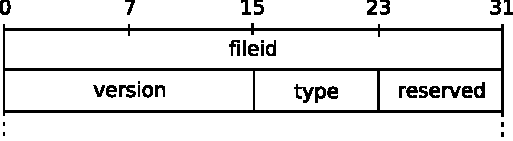
\includegraphics[width=0.7\textwidth]{header-main.pdf}
	\caption{Structure of the main file header}
	\label{fig:header-main}
\end{figure}

The main file header format is made as simple as possible to allow future extensions to be made without breaking backwards compatibility.
In every DECS formatted file the 8 first bytes of the file are occupied by the main header as shown in Table \ref{tab:header-main} and Figure \ref{fig:header-main}.
Currently only the first byte of the version field is used.
In a future versions both bytes in the version field are planned to be ASCII characters so that a separate ASCII format can be defined.
The type field indicates how the data following the header will look like.
When the ASCII format is defined it will probably use the two ASCII characters ``M'' and ``R'' to indicate the type of file.

%The version field indicates the lowest possible file format version implemented which will be able to read this version of the file.
%This means that if the file format version implemented in a program is lower than the compat field it will not be able to read and process it correctly.


\subsubsection{Matrix file format}

When the type field in the main header is 0 then the file contains an exact cover matrix.
It also means that the 40 bytes following the main header is part of the matrix file format header.
The full structure of the matrix header is shown Table \ref{tab:header-matrix} and Figure \ref{fig:header-matrix}.

The DLX algorithm does not use the column and row names that \texttt{name\_off} points to or the problem ID and the problem specific information.
This information can be used by the BOINC client to display graphical information during the computation.
For example it can use the problem ID to identify the correct transform, and when the DLX algorithm finds a solution it can run the reverse transform and display the solution graphically.
As an example the $n$-queens problem could update the screen every 5 second with the last solution found along with the total number of solutions found at that point.
BOINC has built-in support for OpenGL rendering and the solutions could be displayed as part of a special BOINC screen saver.
The structure of the problem information is up to the developers of the problem specific library to determine.
The only requirement is that the first 4 bytes must contain the size of the data (including the value itself) as an unsigned 32-bit integer.

One special note should be made of the bit flags at offset 44.
The least significant bit (LSB) in the bit flag value is the ``conserve bandwidth`` flag.
When the conserve bandwidth flag is set only the number of solutions should be stored in the DECS result file when the problem has been solved.
If the conserve bandwidth flag is not set then every single solution is stored in the result file.
This setting can be overridden by the presence of a special command line argument.
The rest of the bits are yet to be assigned a value and meaning.

\begin{table}[tbp]
	\centering
	\begin{tabular}{|r|r|p{3.2in}|}
		\hline
		\bf Offset & \bf Length & \bf Description \\ \hline
		8  & 4 & \texttt{cols\_num} - Number of columns $> 1$. \\ \hline
		12 & 4 & \texttt{rows\_num} - Number of rows $> 1$. \\ \hline
		16 & 4 & \texttt{elems\_num} - Number of non-zero values in the matrix $> 1$. \\ \hline
		20 & 4 & \texttt{elems\_off} - Byte offset to the matrix element entries. Should never be 0. \\ \hline
		24 & 4 & \texttt{secol\_off} - Byte offset to the secondary column list. 0 if unavailable. \\ \hline
		28 & 4 & \texttt{init\_off} -  Byte offset to the initialization vector. 0 if unavailable. \\ \hline
		32 & 4 & \texttt{name\_off} - Byte offset to the column and row name list. 0 if unavailable. \\ \hline
		36 & 4 & \texttt{prob\_id} - Problem ID. Each problem type has a unique ID so that the correct transform can be chosen and the problem specific information can be decoded. \\ \hline
		40 & 4 & \texttt{prob\_off} - Byte offset to problem specific information. 0 if unavailable. \\ \hline
		44 & 4 & \texttt{flags} - Bit flags for various purposes. \\ \hline
	\end{tabular}
	\caption{Matrix file header format. Offset and length in bytes.}
	\label{tab:header-matrix}
\end{table}

\begin{figure}[tbp]
	\centering
	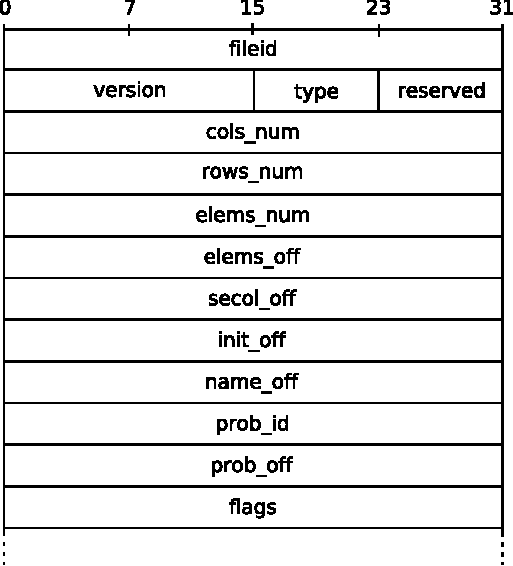
\includegraphics[width=0.7\textwidth]{header-matrix.pdf}
	\caption{Structure of the matrix file header combined with the main header}
	\label{fig:header-matrix}
\end{figure}


\subsubsection{Result file format}

If the type field in the main header is 1 then the file contains the results of an exact cover problem.
The size of the result header is 16 bytes as shown in Table \ref{tab:header-result} and Figure \ref{fig:header-result}.

When the DLX algorithm has solved an exact cover problem it stores the results in a file using the result file format.
If the conserve bandwidth flag is set in the matrix file then \texttt{results\_off} will be zero.
This indicates that no solutions are stored in the file.

The structure of the data pointed to by many of the byte offsets are simple lists that consists of unsigned 32-bit integers.
This format is used by the solution list (\texttt{results\_off}), matrix element list (\texttt{elems\_off}), secondary column list (\texttt{secol\_off}) and the initialization vector list (\texttt{init\_off}).
The first value $n$ is the size of the list indicating how many unsigned 32-bit integers it contains.
Reading the following $n$ values ($4n$ bytes) provides all the elements of the list.
The solution list and matrix element list are actually a sequence of lists where each list represents one solution (set of rows) or one row in the matrix (set of columns numbers for elements with non-zero values).
By using the value read from the respective header fields \texttt{results\_num} or \texttt{rows\_num} the correct number of lists can be obtained from the file.

\begin{table}[htbp]
	\centering
	\begin{tabular}{|r|r|p{3.2in}|}
		\hline
		\bf Offset & \bf Length & \bf Description \\ \hline
		8  & 4 & \texttt{results\_num} - Number of results. \\ \hline
		12 & 4 & \texttt{results\_off} - Byte offset to the list of solutions. 0 if unavailable. \\ \hline
		16 & 4 & \texttt{prob\_id} - Problem type ID. Each problem type has a unique ID so that the correct transform can be chosen and the problem specific information can be decoded. \\ \hline
		20 & 4 & \texttt{prob\_off} - Byte offset to problem specific information. 0 if unavailable. \\ \hline
	\end{tabular}
	\caption{Result file header format. Offset and length in bytes.}
	\label{tab:header-result}
\end{table}

\begin{figure}[htbp]
	\centering
	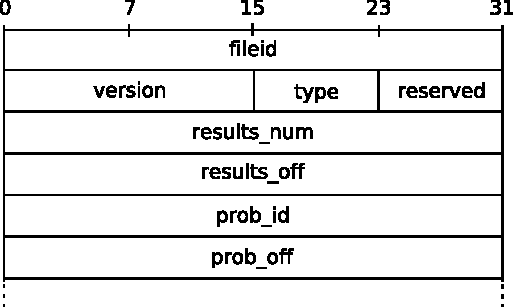
\includegraphics[width=0.7\textwidth]{header-result.pdf}
	\caption{Structure of the result file header combined with the main header}
	\label{fig:header-result}
\end{figure}



\section{libdecs}


\subsection{Modes of operation}

DECS has two basic modes of operation regarding how it handles the return values in the system.
In the first mode each client will store and forward all the solutions it finds back to the BOINC server.
This provides the calling application with the full set of solutions so that it can run a detailed analysis on them or save them for later use.
For problems which generates a very large number of solutions this approach can cause a huge strain on the system.
The storage and bandwidth capacities of the computing nodes and the BOINC server would quickly become a bottleneck if there are too many solutions.
In extreme cases it might even cause some of the solutions to never be returned because the system is unable to handle the load.
A policy of not accepting overly large problem matrices could be implemented to prevent this problem.

The second mode of operation will discard the actual results, but instead keep a count on how many solutions has been found.
When a matrix has been solved it only returns the value holding the number of solutions to the server.
This drastically reduces the bandwidth and storage requirements for the clients and servers, but it also makes it impossible to analyze the final solutions.
This is the default mode used by the $n$-queens library because there we are usually not interested individual solutions.
Instead we only want to know the total number of solutions.

A possible extension to this would be to add other return values than the number of solutions.
Each solution the DLX algorithm finds could be further analyzed so that other aspects of the solutions could be returned.

%The main purpose of libdlx is to parse a file with the problem matrix and to apply the DLX algorithm in order to solve it.
%The theory behind the DLX algorithm has been covered in Chapter \ref{dancing_links}.
%Here we will look at the external interface to libdlx and some of its internals.


\subsection{Building the boolean matrix}
\label{matrix_construction}

Before the DLX algorithm can be started the matrix needs to be read from a file and the data structures must be initialized.
Each non-zero element in the matrix is a quad-linked node in a circular quad-linked structure.

To construct the matrix data structure we have some special column objects.
Before the nodes are added a root node is created which is the basis for the entire structure.
To the right of the root node all the column header nodes are added in the order of increasing column indices.
Algorithm~\ref{alg:columns} shows how the circular doubly-linked column list is created.
It starts by creating the root node $R$ onto which all the column nodes are attached.
Take special note of how the secondary column objects are linking to themselves on line 10 and 11.
\begin{algorithm}[htbp]
	\caption{Create the circular doubly-linked list of columns.}
	\label{alg:columns}
	\algsetup{indent=6mm}
	\begin{distribalgo}[1]
		\STATE $R \leftarrow$ new column object
		\STATE $T \leftarrow R$
		\FOR{$i \leftarrow 1$ \textbf{to} the value of the \texttt{cols\_num} field}
			\STATE $C \leftarrow$ new column object with index $i$
			\IF{column $i$ is a primary column}
				\STATE $C.left \leftarrow T$  \COMMENT{Add primary column header}
				\STATE $T.right \leftarrow C$
				\STATE $T \leftarrow C$
			\ELSE
				\STATE $C.left \leftarrow C$  \COMMENT{Add secondary column header}
				\STATE $C.right \leftarrow C$
			\ENDIF
			\STATE $H[i] \leftarrow C$
		\ENDFOR
		\STATE $R.left \leftarrow T$
		\STATE $T.right \leftarrow R$
	\end{distribalgo}
\end{algorithm}

To initialize the data structure the nodes must be added row by row by reading them from the left to the right side.
The algorithm starts with the top row and works its way down to the bottom.
It also makes use of the column header array $H$ which was initialized in Algorithm \ref{alg:columns}.

\begin{algorithm}[htbp]
	\caption{Create the circular quad-linked node structure.}
	\label{alg:nodes}
	\algsetup{indent=6mm}
	\begin{distribalgo}[1]
		\FOR{$i \leftarrow 1$ \textbf{to} the value of the \texttt{rows\_num} field}
			\FOREACH{column index $j$ in row $i$}
				\STATE $N \leftarrow$ new node object with row index $i$
				\STATE $C \leftarrow H[j]$
				\STATE $N.column \leftarrow C$
				\STATE $C.size \leftarrow C.size + 1$  \COMMENT{Increment column size}
				\STATE $N.up \leftarrow C.up$  \COMMENT{Add element to column list}
				\STATE $N.down \leftarrow C$
				\STATE $C.up.down \leftarrow N$
				\STATE $C.up \leftarrow N$
				\IF{$T$ is set}
					\STATE $N.left \leftarrow T$  \COMMENT{Add element to row list}
					\STATE $N.right \leftarrow T.right$
					\STATE $T.right.left \leftarrow N$
					\STATE $T.right \leftarrow N$
				\ELSE
					\STATE $N.left \leftarrow N$  \COMMENT{First node in a row}
					\STATE $N.right \leftarrow N$
				\ENDIF
				\STATE $T \leftarrow N$
			\ENDFOR
			\STATE Unset $T$
		\ENDFOR
	\end{distribalgo}
\end{algorithm}




\chapter{Testing and simulation}
\label{testing}

% Description of what tests has been performed.


\section{Simulation}

%This Petri net model, simulation and analysis project has been inspired by the author's current work in the Generic Distributed Exact Cover Solver (DECS) \cite{decs-web} project.
%DECS details the implementation of a distributed computing system to solve exact cover problems by using Donald Knuth's Dancing Links (DLX) \cite{knuth00dancing} algorithm.
%Figure \ref{fig:architecture} provides the basic architecture of this distributed computing system.

DECS mainly works by dividing a problem into smaller pieces and through BOINC \cite{boinc} it distributes these pieces to a collection of client systems.
BOINC also handles the result collection process.
In BOINC the clients send HTTP GET and POST messages to a web server in order to download more work and upload the results.
We wish to simulate this system by constructing a Petri net model which represents a simplified version of DECS.
Petri net, invented in 1962 by Carl Adam Petri \cite{Petri62, Petri66}, is used to model and simulate discrete-event systems.


\subsection{Model}

The Petri net model is based on the architecture as shown in Figure \ref{fig:architecture}.
In order for the simulation to be useful the complete request/response cycle has been modeled.
The firing times of the transitions have been determined by research and testing.


\subsubsection{Assumptions}

To begin with a few assumptions are made regarding the system being modeled.
This is done in order to make the model simple and easy to understand.
Because we are dealing with a distributed system we need to be aware of the most common pitfalls we might encounter.
From ``The eight fallacies of distributed computing'' \cite{distributed-fallacies} the following assumptions apply to our model:

\begin{itemize}
	\item The network is reliable.
	\item Topology does not change.
\end{itemize}

We assume that all the hardware and the software in the distributed system is reliable.
Without this assumption we would have to take into account all sorts of failure scenarios which would cause the Petri net model to become overly complex.
The model also assumes that the network topology does not change significantly.
BOINC itself can deal with several different changes to topology, like disconnected clients and wireless roaming clients, etc., but to make the model simple we assume that the clients are always reachable through the network.

However, there are some of the eight fallacies we do NOT make assumptions about or which do not apply to this project:

\begin{itemize}
	\item Latency is zero.
	\item Bandwidth is infinite.
	\item The network is secure.
	\item There is one administrator.
	\item Transport cost is zero.
	\item The network is homogeneous.
\end{itemize}

Zero latency is not assumed because the latency of the distributed system is modeled by the firing time of each of the transitions.
In the cases where it counts we do not assume infinite bandwidth.
However, it is difficult to accurately model both the bandwidth limitation and the latency between the clients and the server without making the model significantly harder to understand.
The current solution is a compromise between accuracy and readability.
BOINC handles all the network communication and carries the burden of securing the distributed system against attacks.
These security mechanisms are not modeled because they have no direct impact on the performance of the system.
The ``one administrator'' and ``zero transport cost'' assumptions fall outside the scope of this report.
The way the system is administered and the infrastructure costs are not our concern.
As far as BOINC goes it does not care what platform the server or clients run because it is able to supports most major operating systems and hardware platforms.
Some additional assumptions are presented later under the sections they belong to.


\subsubsection{Server model}

We begin by first modeling the server in this distributed computing system.
It is assumed that there is only one server, even though BOINC in practice can support more than one.
The server has two ``pipelines'' so to speak: The request pipeline and the response pipeline.
In Figure \ref{fig:petri-server} shows the complete server model.

The request pipeline begins with the place $p_{req}$ onto which an application may submit a specific exact cover problem to be processed by DECS.
The specific problem is then transformed into a more generic form by the transition $t_{tr}$ before it is placed in $p_{div}$.
From there the problem is divided into several smaller problems by $t_{div}$ and the resulting pieces\footnote{BOINC uses the term ``work units'' instead of pieces, but it is essentially the same thing.} are placed in $p_{dist}$ to be distributed to the clients.
The weight, $m$, of the arc from $t_{div}$ to $p_{dist}$ is the number of pieces the problem is divided into.

The response pipeline starts with the place $p_{col}$ where the solutions from the clients are placed.
When all the solutions have arrived they are merged together by $t_{mrg}$ and the resulting solution is placed in $p_{rtr}$.
The weight of the arc from $p_{col}$ to $t_{mrg}$ will also have to be $m$ in order to ensure that the merging process does not take place before all the solutions has arrived.
From $p_{rtr}$ the generic solution is transformed back into the domain of the specific problem by $t_{rtr}$ and returned to the application in $p_{res}$.

\begin{figure}[htbp]
	\centering 
	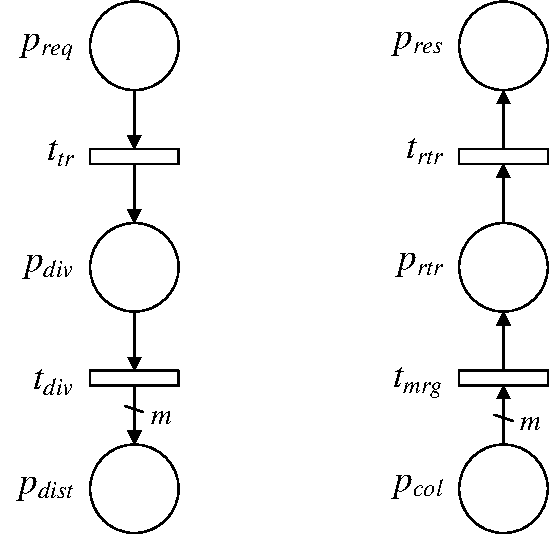
\includegraphics[width=0.6\textwidth]{petri-server.pdf}
	\caption{Petri net for the distributed computing server}
	\label{fig:petri-server}
\end{figure}


\subsubsection{Network model}

\begin{figure}[htbp]
	\centering 
	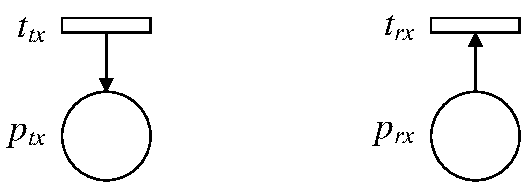
\includegraphics[width=0.6\textwidth]{petri-network.pdf}
	\caption{Petri net for the distributed computing network}
	\label{fig:petri-network}
\end{figure}

In an attempt to model the bandwidth limitation on the server side the Petri net in Figure \ref{fig:petri-network} has been designed.
It is a primitive bandwidth throttling device and with the correct firing times it should be able to regulate the flow of data coming from and going to the server.
$t_{tx}$ and $p_{tx}$ model the transmit limit and $t_{rx}$ and $p_{rx}$ model the receive limit.
It is assumed that the network communication channel is full duplex\footnote{Full duplex allows data to be sent and received at the same time.} and that the combined network bandwidth of all the connected clients is equal to or larger than the bandwidth on the server side.
In other words we assume that the bottleneck is on the server side, which is true in most cases where the number of clients is high.
The individual bandwidth limitations for each client and the complete operation of the TCP/IP and HTTP protocols are not modeled.


\subsubsection{Client model}

\begin{figure}[htbp]
	\centering 
	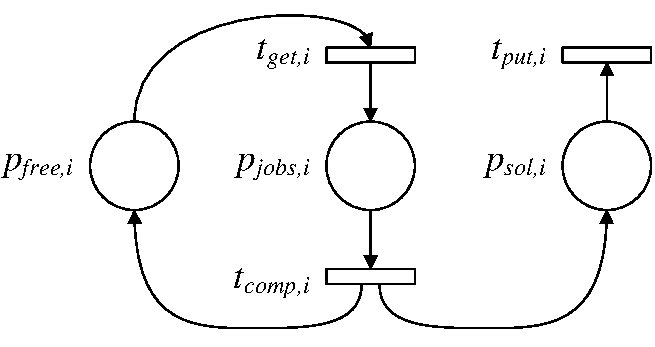
\includegraphics[width=0.7\textwidth]{petri-client.pdf}
	\caption{Petri net for a single distributed computing client}
	\label{fig:petri-client}
\end{figure}

Figure \ref{fig:petri-client} shows the Petri net model of a single computing client.
To model a system with more than one client the client model is duplicated as many times as there are clients.
To identify each client they are given a number $i$ from $1$ to $n$.
When $t_{get,i}$ is fired the HTTP GET request is send to the server and a piece of the problem is returned to the client and placed in $p_{jobs,i}$, which is a job queue.
$t_{comp,i}$ is the computing program which processes each job from $p_{jobs,i}$ one at a time.
This model assumes that the computing program is only able to process one problem at the same time, even on multi-processor systems.
When a computation is complete the resulting solution is placed in $p_{sol,i}$ and then sent to the server by $t_{put,i}$.
$p_{free,i}$ is used to control the number of simultaneous pieces that a client can work on at the same time.
The get and put operations are assumed to be running in a separate thread so that they do not significantly impact the running time of a computation.


\subsubsection{Petri net definition}

A Petri net graph is a weighted bipartite graph $(P, T, A, w)$.
$P$ is the set of places, $T$ is the set of transitions, $A$ is the set of arcs and $w$ is the arc weight function.
A Petri net model of the system with a single client is shown in Figure \ref{fig:petri-system}.
If additional clients are added the complexity steadily increases as the client model is duplicated and each client is connected to $p_{tx}$ and $p_{rx}$.
Below we have defined the Petri net model as shown in the figure.

\begin{align*} 
P &= \left\{p_{req}, p_{res}, p_{rtr}, p_{div}, p_{dist}, p_{col}, p_{tx}, p_{rx}, p_{free}, p_{jobs}, p_{sol}\right\} \\
T &= \left\{t_{tr}, t_{rtr}, t_{div}, t_{mrg}, t_{tx}, t_{rx}, t_{get,1}, t_{comp,1}, t_{put,1}\right\} \\
A &= \{(p_{req}, t_{tr}), (t_{tr}, p_{div}), (p_{div}, t_{div}), (t_{div}, p_{dist}), (p_{col}, t_{mrg}), (t_{mrg}, p_{rtr}), \\
&(p_{rtr}, t_{rtr}), (t_{rtr}, p_{res}), (p_{dist}, t_{tx}), (t_{rx}, p_{col}), (p_{tx}, t_{get,1}), (t_{put,1}, p_{rx}), \\
&(t_{get,1}, p_{jobs,1}), (p_{jobs,1}, t_{comp,1}), (t_{comp,1}, p_{free,1}), (p_{free,1}, t_{get,1}), \\
&(t_{comp,1}, p_{sol,1}), (p_{sol,1}, t_{put,1})\} \\
w&(t_{div}, p_{dist}) = w(p_{col}, t_{mrg}) = m \\
\end{align*}

\begin{figure}[htbp]
	\centering 
	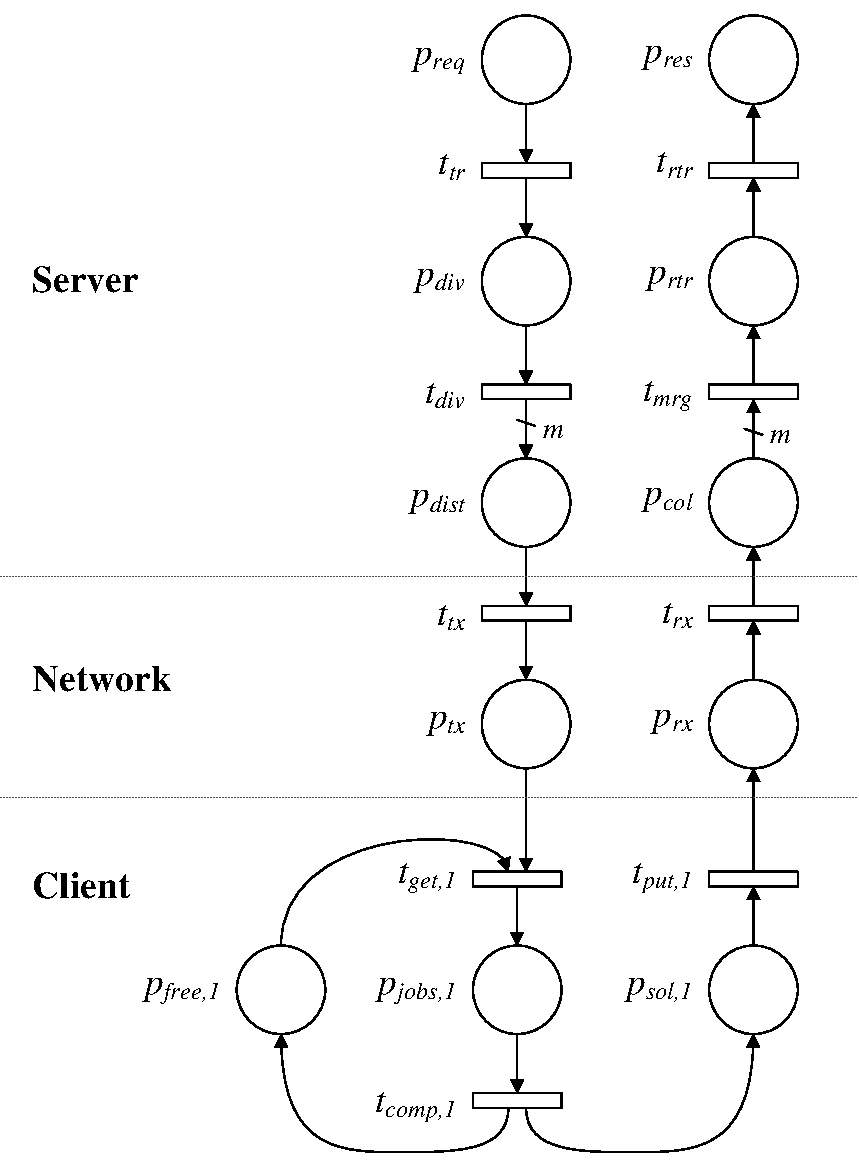
\includegraphics[width=1.0\textwidth]{petri-system.pdf}
	\caption{Petri net model of the DECS system with a single client connected}
	\label{fig:petri-system}
\end{figure}


\subsection{Simulation}

GPenSIM \cite{gpensim} version 2.1 is used in the modeling and simulation of this distributed computing system.
GPenSIM is a software package for MATLAB which enables one to use all the powerful facilities for statistics and plotting which MATLAB is known for.


\subsubsection{Simulation parameters}

To fully define the model a set of different parameters has to be defined.
These parameters are the firing times of the transitions, arc weights, number of clients and the initial dynamics\footnote{The initial dynamics/markings is the number and location of tokens at the start of the simulation.}.

To be able to find the correct parameters we need to specify what problem we want DECS to solve.
Lets say that we want to solve the 20-queens problem.
It should take about 12 hours of CPU time to solve this problem according to the NQueens@Home project \cite{nqueensathome}.
Although they are using a specialized algorithm instead of the DLX algorithm used by DECS, we assume that the running time is about the same.
In reality the DLX algorithm is significantly slower than the algorithm used by the NQueens@Home project.

The number of clients is chosen to be $n = 12$, meaning that if this was an ideal system the problem would be solved in 1 hour.
Each client should use around 10 minutes to solve each piece of the problem so the problem is divided into $m = 72$ pieces.
The transformation of the specific 20-queens problem to the DLX matrix takes 160 milliseconds so the firing time for $t_{tr}$ is 0.160 seconds.
The reverse transform, given that the number of solutions is about 39 billions, takes 39 seconds so that the firing time for $t_{rtr}$ is 39.
The system can also be modeled so that only a value containing the number of solutions is returned from the clients, instead of returning the complete set of solutions.
Dividing the problem into 72 pieces in DECS gives a firing time of 0.12 seconds for $t_{div}$.
Merging the solutions in $t_{mrg}$ results in a firing time of 7.2 seconds.
Since we model the solution of only one problem we have to place one initial token in $p_{req}$.

Each of the problem pieces are 100 kilobit large and the server has a upstream bandwidth of 400 kbps (kilobit per second).
This gives a throughput of 4 pieces per second which means that the firing time of $t_{tx}$ must be 0.25 second.
$p_{tx}$ should have a maximum number of tokens so that it better reflects the correct bandwidth when no more HTTP GET requests are being issued by the clients.
We choose to set the maximum limit to 4, which is the maximum number of pieces that can be send each second.
The downstream bandwidth of the server is 2000 kbps and each of the solutions has been compressed down to 8000 kilobit.
The rate of packets downstream will be 0.25 per second, which results in a 4 second firing time of $t_{rx}$.

Each of the clients has an average round trip time (RTT) to the server of about 100 milliseconds.
For HTTP this gives a latency of $2 \times RTT +$ the time it takes to transfer the file.
The file transfer times has already been accounted for by $t_{tx}$ and $t_{rx}$.
Since the RTT will usually vary a bit we use a normal distribution with a mean of 200 milliseconds ($2 \times RTT$) and a standard deviation of 20 to generate random firing times for $t_{get}$ and $t_{put}$.
The firing time of $t_{comp}$ is a uniform distribution with a minimum of 8 minutes and a maximum of 12.
We also put two tokens in $p_{free}$ to allow each client to retrieve two pieces of work from the server initially.


\subsection{Results}

From Figure \ref{fig:initdist} you can see that the primitive bandwidth throttling is doing its job.
It takes about 7 seconds to distribute the initial 24 pieces\footnote{Each of the 12 clients requests 2 pieces each to begin with because they have two tokens in $p_{free}$.} from $p_{dist}$ to the clients.

\begin{figure}[htbp]
	\centering 
	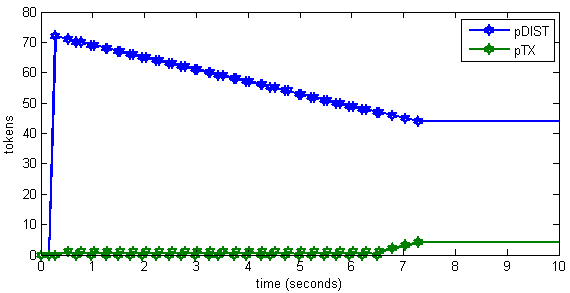
\includegraphics[width=1.0\textwidth]{initial_distribution.png}
	\caption{Initial distribution during the first 10 seconds}
	\label{fig:initdist}
\end{figure}

A complete simulation in GPenSIM takes 364 steps and depending on the random timing it finishes around 67 minutes.
Figure \ref{fig:complete_sim} shows a complete simulation which only took 63 minutes.
You can clearly see the stages when each of the clients finish their work and request a new piece from the server.
Another simulation shown in Figure \ref{fig:complete_sim2} with the same parameters appears to have distributed the distribute and collect operations more evenly in time.
This would no doubt have caused less stress on the server and its bandwidth, but unfortunately it also hurts performance as it used 67 minutes in total to solve the problem.

\begin{figure}[htbp]
	\centering 
	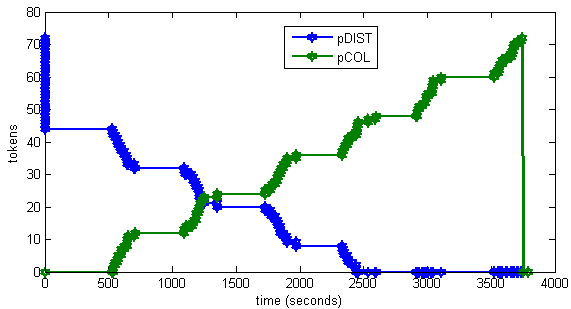
\includegraphics[width=0.9\textwidth]{complete_sim.png}
	\caption{Complete simulation of the distribution and collection completed in 63 minutes}
	\label{fig:complete_sim}
\end{figure}

\begin{figure}[htbp]
	\centering 
	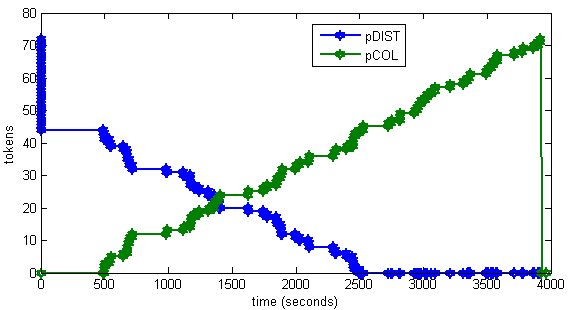
\includegraphics[width=0.9\textwidth]{complete_sim2.png}
	\caption{Another simulation of the distribution and collection completed in 67 minutes}
	\label{fig:complete_sim2}
\end{figure}

By multiplying the number of clients by 4 so that $n = 48$ one might expect the total time to solve the problem would be reduced by 75\%.
However, as seen by Figure \ref{fig:sim-48clients} it takes about 24 minutes, which is only a 64\% reduction (relative to a 67 minute simulation with 12 clients).
Ideally it should have taken 15 minutes, but with the increased amount of clients the limited bandwidth on the server is starting to become a bottleneck.
The number of pieces is also a problem as there are now 1.5 pieces for each client, and as a result about half of the clients have no work to process during the last stage.

\begin{figure}[tbp]
	\centering 
	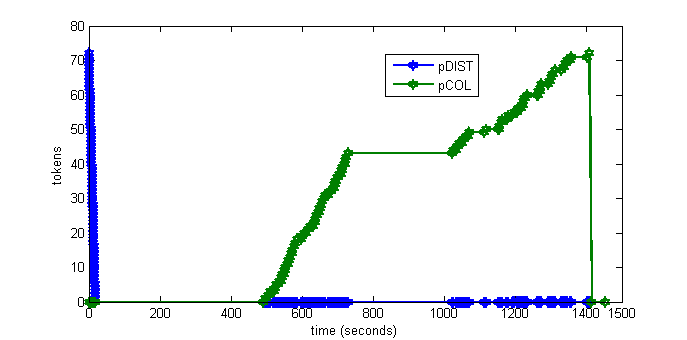
\includegraphics[width=0.9\textwidth]{sim-48-clients.png}
	\caption{Simulation of the distribution and collection with 48 clients}
	\label{fig:sim-48clients}
\end{figure}

A slight optimization can be done by reducing the number of tokens in $p_{free,i}$ from 2 to 1.
This will allow the clients who completes the first piece fastest to request a second piece and start working on it.
This adjustment will cause the 24 slowest clients to not get any work.
Figure \ref{fig:sim-48clients-1free} shows the result of this simulation which took about 22 $1/2$ minute.

\begin{figure}[tbp]
	\centering 
	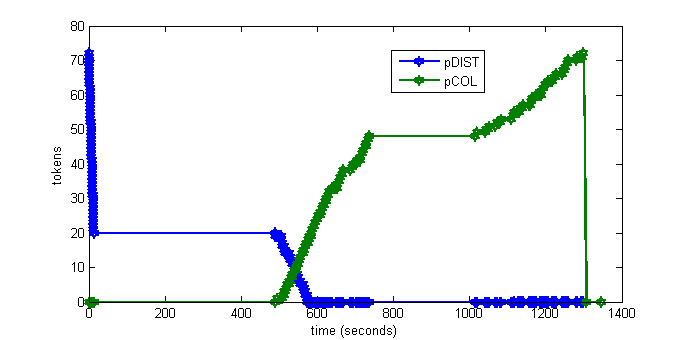
\includegraphics[width=0.9\textwidth]{sim-48-clients-1-free.png}
	\caption{Simulation of the distribution and collection with 48 clients and 1 token in $p_{free,i}$}
	\label{fig:sim-48clients-1free}
\end{figure}


The main challenge in modeling this system is the distribution and collection mechanism and making sure that the latency and bandwidth limitations were preserved.



%\section{Performance}
% TODO: Semi-Important - Write a bit about performance of the dance program.



\chapter{Conclusion}
\label{conclusion}

% Description of important/interesting implementation details.

\section{Future work}

\subsection{Sub-bit precision packing}

To make the file format explanation easy to understand the conventional bit packing technique was chosen over sub-bit precision packing.
With sub-bit precision packing we can achieve an even better file size reduction at the expense of a few more CPU cycles.
This is especially important for problems having very large DLX matrices.
By implementing this extension to the conventional technique we will increase the performance of the system.




% BibTeX compiles the bibliography
\phantomsection
\addcontentsline{toc}{chapter}{\bibname}
\bibliographystyle{custom-r2}  % custom bibliography style
\bibliography{local,nqueens}  % import local.bib

\end{document}
